\chapter{Limit}
The events passing the kinematical selection are compared with expectations
from Standard Model background sources. The number of expected events from
the signal Monte Carlo is shown in table~\ref{tab:signal_yields_sum}. The
backgrounds are compared to the observed event yields in
table~\ref{tab:background_yields_sum}.
        \begin{table}[pbt]
            \centering
            \begin{tabular}{l *3{r@{$\pm$}l}}
                
\toprule
dataset & \multicolumn{2}{c}{same-sign, 2 jets}& \multicolumn{2}{c}{preselection}& \multicolumn{2}{c}{razor} \\
\midrule
T53 400& 211.10 & 10.73& 151.16 & 7.73& 54.34 & 2.88\\
T53 450& 104.52 & 5.31& 77.93 & 3.98& 41.34 & 2.15\\
T53 500& 52.76 & 2.68& 40.09 & 2.04& 25.61 & 1.32\\
T53 550& 28.53 & 1.45& 22.47 & 1.14& 16.22 & 0.83\\
T53 600& 15.34 & 0.78& 12.07 & 0.61& 9.39 & 0.48\\
T53 650& 8.65 & 0.44& 6.87 & 0.35& 5.57 & 0.28\\
T53 700& 5.00 & 0.25& 3.98 & 0.20& 3.37 & 0.17\\
T53 750& 2.97 & 0.15& 2.35 & 0.12& 2.01 & 0.10\\
 \\
\bottomrule

            \end{tabular}
            \caption{Signal Monte Carlo yields for the various mass points
            in the three decay channels. Statistical and systematic uncertainties are shown.}
            \label{tab:signal_yields_sum}
        \end{table}


        \begin{table}[pbt]
            \centering
            \begin{tabular}{l *3{r@{$\pm$}l}}
                
\toprule
dataset & \multicolumn{2}{c}{same-sign, 2 jets}& \multicolumn{2}{c}{preselection}& \multicolumn{2}{c}{razor} \\
\midrule
WW, WWW& 2.86 & 6.67& 0.22 & 0.45& 0.05 & 0.14\\
TTZ, TTW& 3.97 & 9.31& 1.33 & 3.20& 0.31 & 0.71\\
WZ, ZZ& 8.57 & 6.17& 0.41 & 0.36& 0.09 & 0.08\\
\midrule
total MC& 15.40 & 13.01& 1.95 & 3.25& 0.45 & 0.73\\
charge misid& 18.38 & 4.81& 0.22 & 0.17& 0.04 & 0.03\\
non-prompt & 34.99 & 1.91& 2.27 & 0.48& 0.12 & 0.11\\
observed & \multicolumn{2}{c}{77}& \multicolumn{2}{c}{3}& \multicolumn{2}{c}{2} \\
\bottomrule

            \end{tabular}
            \caption{Expected backgrounds and observed yields for different
            cuts in the \E\E\ channel. Statistical and systematic uncertainties are
            shown.}
            \label{tab:background_yields_ee}
        \end{table}

        \begin{table}[pbt]
            \centering
            \begin{tabular}{l *3{r@{$\pm$}l}}
                
\toprule
dataset & \multicolumn{2}{c}{same-sign, 2 jets}& \multicolumn{2}{c}{preselection}& \multicolumn{2}{c}{razor} \\
\midrule
WW, WWW& 6.63 & 6.67& 0.48 & 0.45& 0.16 & 0.14\\
TTZ, TTW& 9.13 & 9.31& 3.39 & 3.20& 0.71 & 0.71\\
WZ, ZZ& 17.45 & 6.17& 1.12 & 0.36& 0.19 & 0.08\\
\midrule
total MC& 33.21 & 13.01& 4.99 & 3.25& 1.07 & 0.73\\
charge misid& 4.66 & 4.81& 0.60 & 0.17& 0.11 & 0.03\\
non-prompt & 50.61 & 3.41& 5.44 & 1.20& 0.25 & 0.28\\
observed & \multicolumn{2}{c}{48}& \multicolumn{2}{c}{8}& \multicolumn{2}{c}{2} \\
\bottomrule

            \end{tabular}
            \caption{Expected backgrounds and observed yields for different
            cuts in the \E\M\ channel. Statistical and systematic uncertainties are
            shown.}
            \label{tab:background_yields_emu}
        \end{table}

        \begin{table}[pbt]
            \centering
            \begin{tabular}{l *3{r@{$\pm$}l}}
                
\toprule
dataset & \multicolumn{2}{c}{same-sign, 2 jets}& \multicolumn{2}{c}{preselection}& \multicolumn{2}{c}{razor} \\
\midrule
WW, WWW& 3.78 & 6.67& 0.18 & 0.45& 0.07 & 0.14\\
TTZ, TTW& 5.47 & 9.31& 1.68 & 3.20& 0.39 & 0.71\\
WZ, ZZ& 8.60 & 6.17& 0.45 & 0.36& 0.14 & 0.08\\
\midrule
total MC& 17.86 & 13.01& 2.31 & 3.25& 0.60 & 0.73\\
charge misid& 1.01 & 4.81& 0.01 & 0.17& 0.00 & 0.03\\
non-prompt & 19.64 & 2.06& 3.59 & 0.89& 0.39 & 0.28\\
observed & \multicolumn{2}{c}{32}& \multicolumn{2}{c}{4}& \multicolumn{2}{c}{0} \\
\bottomrule

            \end{tabular}
            \caption{Expected backgrounds and observed yields for different
            cuts in the \M\M\ channel. Statistical and systematic uncertainties are
            shown.}
            \label{tab:background_yields_mumu}
        \end{table}

        \begin{table}[pbt]
            \centering
            \begin{tabular}{l *3{r@{$\pm$}l}}
                
\toprule
dataset & \multicolumn{2}{c}{same-sign, 2 jets}& \multicolumn{2}{c}{preselection}& \multicolumn{2}{c}{razor} \\
\midrule
WW, WWW& 13.28 & 6.67& 0.88 & 0.45& 0.28 & 0.14\\
TTZ, TTW& 18.57 & 9.31& 6.39 & 3.20& 1.41 & 0.71\\
WZ, ZZ& 34.62 & 6.17& 1.97 & 0.36& 0.42 & 0.08\\
\midrule
total MC& 66.47 & 13.01& 9.25 & 3.25& 2.12 & 0.73\\
charge misid& 24.05 & 4.81& 0.83 & 0.17& 0.15 & 0.03\\
non-prompt & 105.24 & 52.80& 11.30 & 5.86& 0.76 & 0.56\\
observed & \multicolumn{2}{c}{157}& \multicolumn{2}{c}{15}& \multicolumn{2}{c}{4} \\
\bottomrule

            \end{tabular}
            \caption{Expected backgrounds and observed yields for different
            cuts in the three decay channels. Statistical and systematic uncertainties are
            shown.}
            \label{tab:background_yields_sum}
        \end{table}

No significant excess over the SM expectations is observed (also see
figures~\ref{fig:mr_data} and~\ref{fig:n_jets_data}), and we can set
lower bounds on the masses of the top partners.

\begin{figure}[htb]
    \centering
    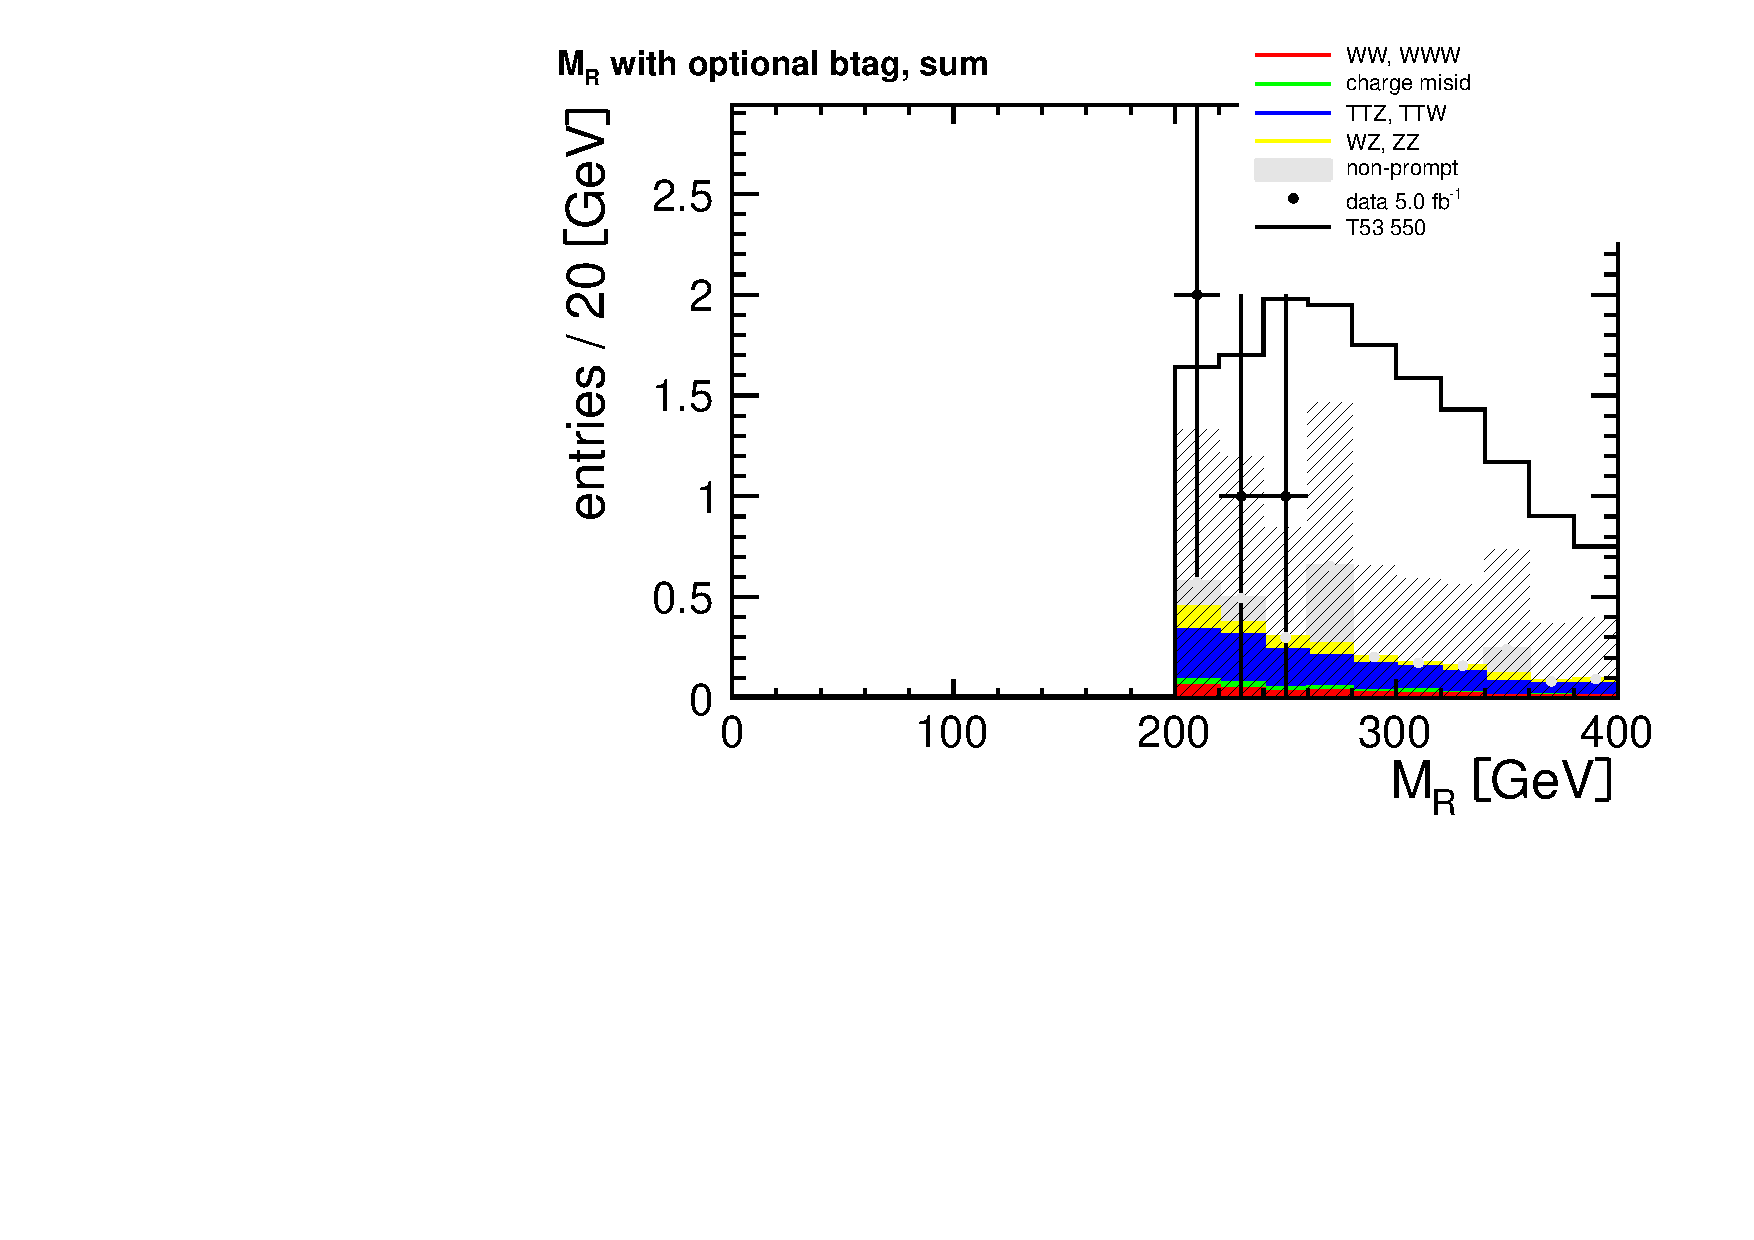
\includegraphics[width=.8\textwidth]{images/pdf/4jets_AND_mr200_AND_r02_AND_had_mass350/mr_optional_btag_sum_1}
    \caption{Distribution of the $M_R$ variable for events in the three decay
        channels, with the final
        selection applied.}
    \label{fig:mr_data}
\end{figure}

\begin{figure}[htb]
    \centering
    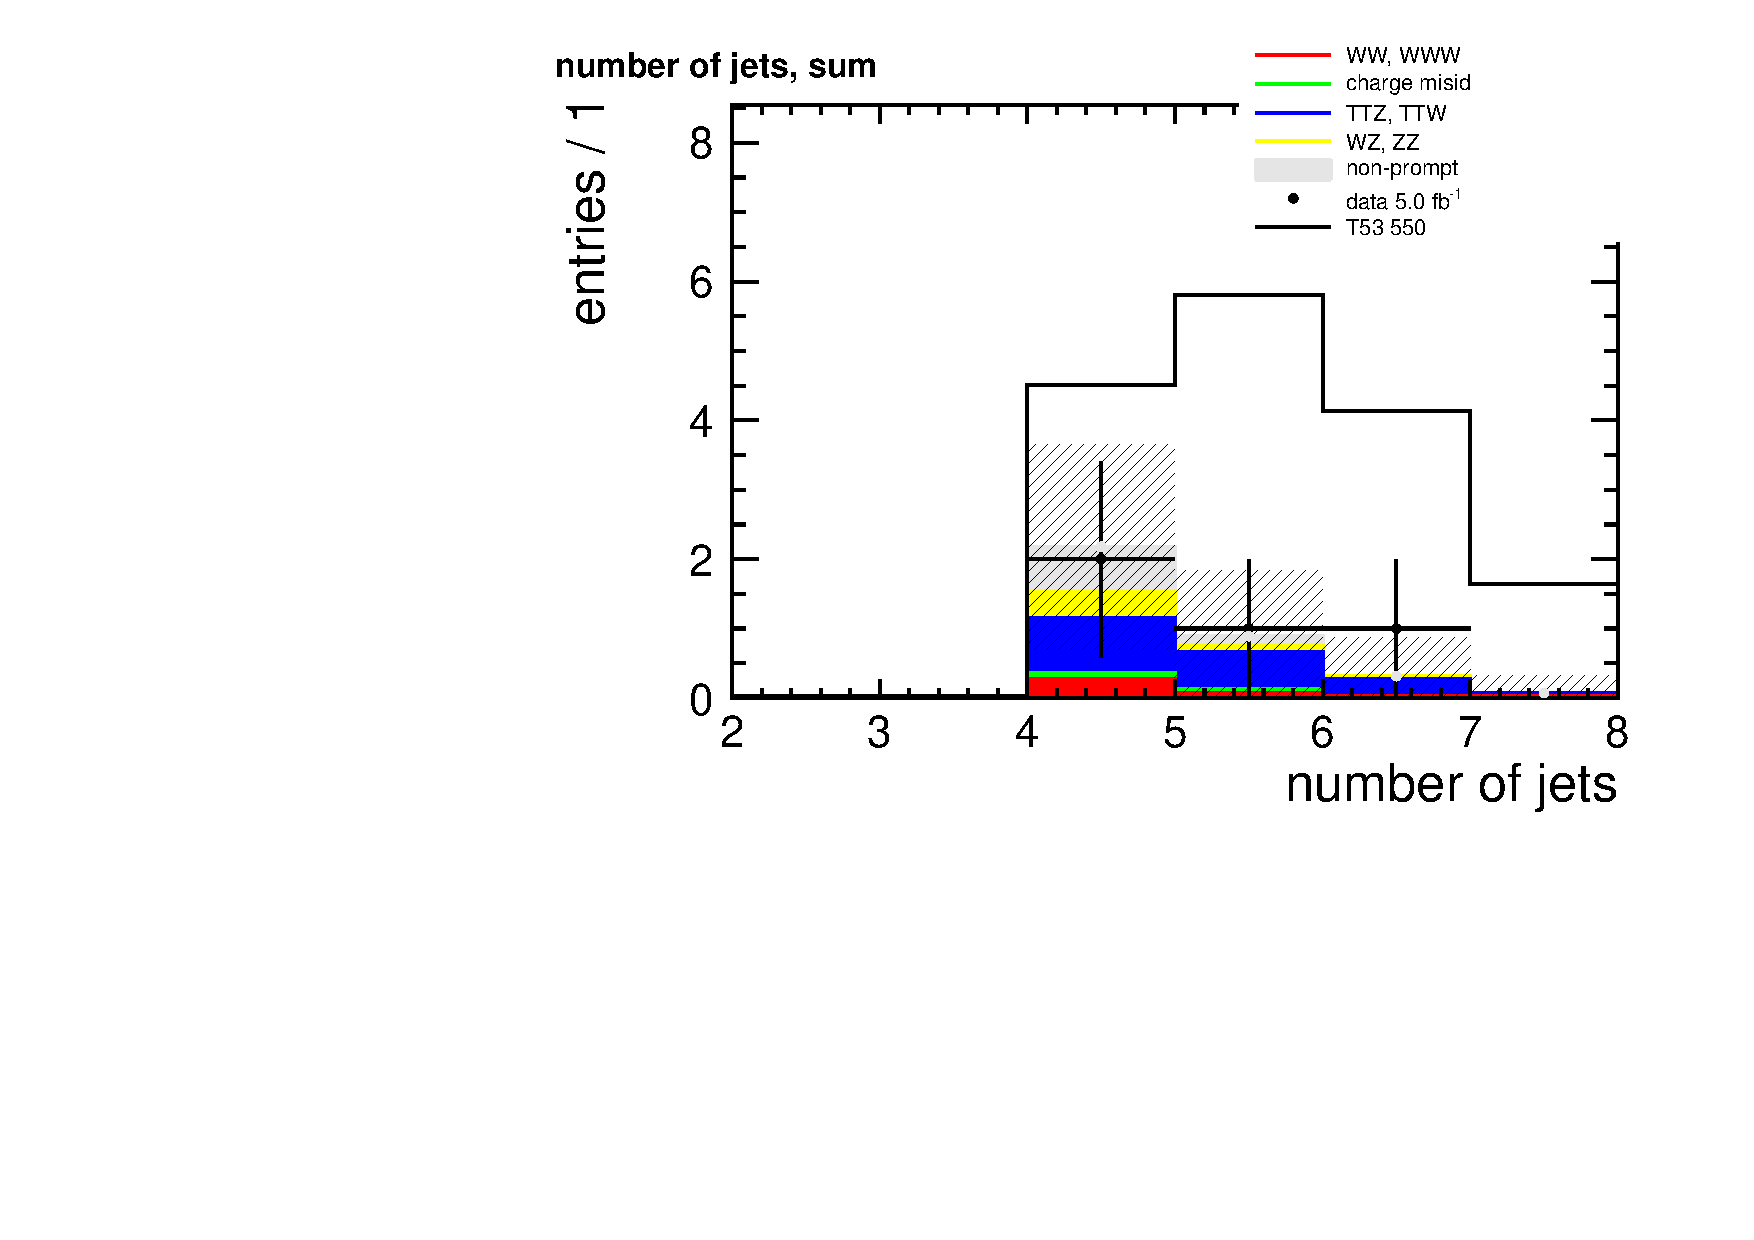
\includegraphics[width=.8\textwidth]{images/pdf/4jets_AND_mr200_AND_r02_AND_had_mass350/n_jets_sum_1}
    \caption{Distribution of the number of jets for events in the three decay
        channels, with the final
        selection applied.}
    \label{fig:n_jets_data}
\end{figure}

Exclusion limits are computed at the 95\% confidence level for an event
counting experiment~\cite{2010acat.confE..57M}.

\section{Calculation of the observed limit}
A modified frequentist method is used at the LHC
experiments~\cite{ATLAS:1379837}, known as the \CLs method.
The test statistic and the treatment of nuisance parameters are described in
this section.

The expected \TP event yields are denoted by $s$, the backgrounds as
$b$. We also introduce the usual \emph{signal strength modifier} $\mu$.
The systematic uncertainties described in~\ref{chap:systematics} are
introduced as nuisance parameters (denoted together as $\theta$) for the number of expected signal and
background events. They become then functions of these parameters
$s(\theta)$ and $b(\theta)$.

The systematic error probability density functions (\emph{pdf}s) $\rho(\theta | \tilde\theta)$ are taken as
gaussians. The mean of the gaussian $\tilde \theta$ is the default value of
the nuisance parameter.
We then re-interpret these systematic errors \emph{pdf}s as posteriors given
by imaginary measurements $\tilde \theta$, as in Bayes' theorem (with flat
$\pi_\theta(\theta)$ priors):
\begin{equation*}
    \rho(\theta|\tilde \theta) \sim p(\tilde \theta | \theta)
    \pi_\theta(\theta)
\end{equation*}
This point of view allows to represent all statistical errors in a
frequentist context: the $p(\tilde \theta|\theta)$ can be used in a sampling
fashion to construct the test statistics, and to constrain the likelihood of
the main measurement.

The procedure for the calculation of the observed limit then includes the
following steps:
\begin{enumerate}
    \item We construct the likelihood function with a Poisson
        distribution:
        \begin{equation*}
            \lhood(\text{data} | \mu, \theta) = \dfrac{(\mu s +
            b)^n}{n!}e^{-\mu s - b} p(\tilde \theta | \theta)
        \end{equation*}
        where \emph{data} represents the actual observed event yields, or
        pseudo-experiments constructed by sampling distributions as
        discussed below.
    \item In order to test the compatibility of the data with the background
        only and signal$+$background hypotheses we build a test statistic
        $\tilde{q}_\mu$  based on the profile likelihood ratio:
        \begin{equation*}
            \tilde{q}_\mu = -2 \log \dfrac{\lhood(\text{data}|\mu,
            \hat{\theta}_\mu)}{\lhood(\text{data}|\hat{\mu},
            \hat{\theta})}
        \end{equation*}
        With the constraint that $0 \leq \hat\mu \leq \mu$. The $0 \leq
        \hat\mu$ is obvious, as the signal rate must be positive, while the
        upper constraint means that fluctuations of the data such that
        $\hat\mu \geq \mu$ are not considered as evidence against the signal
        hypothesis.
        The value of $\hat{\theta}_\mu$ is the conditional maximum
        likelihood estimator of $\theta$, given $\mu$, while the values
        $\hat\mu$ and $\hat\theta$ give the global maximum of the
        likelihood.
    \item The observed value $\tilde{q}_\mu^{\text{obs}}$ for the $\mu$
        under test is calculated.
    \item The values of the nuisance parameters best describing the observed
        data, \ie maximizing the likelihood, are computed for the background
        only and signal$+$background hypotheses. We denote these values as
        $\hat{\theta}_0^{\text{obs}}$ and
        $\hat{\theta}_{\mu}^{\text{obs}}$ respectively.
    \item Monte Carlo pseudo-experiments are made to construct
        \emph{pdf}s $f(\tilde{q}_\mu|\hat{\theta}_{\mu}^{\text{obs}})$ and $f(\tilde{q}_\mu|\hat{\theta}_{0}^{\text{obs}})$ 
        Note that the buisance parameters are fixed for the purposes of
        generating these pseudo-datasets, but are allowed to float in fits
        needed to evaluate the test statistic.
        This gives good coverage properties~\cite{2006sppp.conf..112C}.
    \item We calculate two $p$-values for the $b$-only and $s+b$ hypotheses:
        \begin{align*}
            1 - p_b &= P(\tilde{q}_\mu \geq \tilde{q}_\mu^{\text{obs}} |
            b \text{-only}) &= \int_{q_{0}^{\text{obs}}}^\infty
            f(\tilde{q}_\mu|\hat{\theta}_{0}^{\text{obs}}) \mathrm{\,d}
            \tilde{q}_\mu\\
            p_\mu &= P(\tilde{q}_\mu \geq \tilde{q}_\mu^{\text{obs}} | s+b)
            &= \int_{q_{\mu}^{\text{obs}}}^\infty
            f(\tilde{q}_\mu|\hat{\theta}_{\mu}^{\text{obs}}) \mathrm{\,d}
            \tilde{q}_\mu
        \end{align*}
        and \CLs as the ratio of these two probabilities:
        \begin{equation*}
            \CLs = \dfrac{p_\mu}{1 - p_b}
        \end{equation*}
    \item If for $\mu = 1$, $\CLs \leq 5\%$, we state that the \TP is
        excluded with 95\% confidence level.
        Limits calculated with this \CLs method are known to be
        conservative, \ie the confidence level is actually higher than 95\%.
\end{enumerate}
\section{Calculation of the expected limit}
In order to calculate the expected limit and the bands corresponding to
$1$ and $2\sigma$ fluctuations, we generate many background-only
pseudo-experiments and calculate \CLs as in the observed limit procedure. 

Then, a cumulative probability distribution of results can be plotted, and
the point at which the distribution crosses the quantile of 50\% is the
median expected value, to be taken as the expected limit. The $\pm 1\sigma$
(68\%) is defined by the crossings of the 16\% and 84\% quantiles. Crossings
at the $2.5\%$ and $97.5\%$ define the $\pm 2\sigma$ band.

\section{Results}
The event yields from the three decay channels are
combined when setting the limits.
The expected and observed limits are shown in
figure~\ref{fig:limit}.
The expected limit is~\unit[658]{GeV}, the observed limit
is~\unit[633]{GeV}.

\begin{figure}[htb]
    \centering
    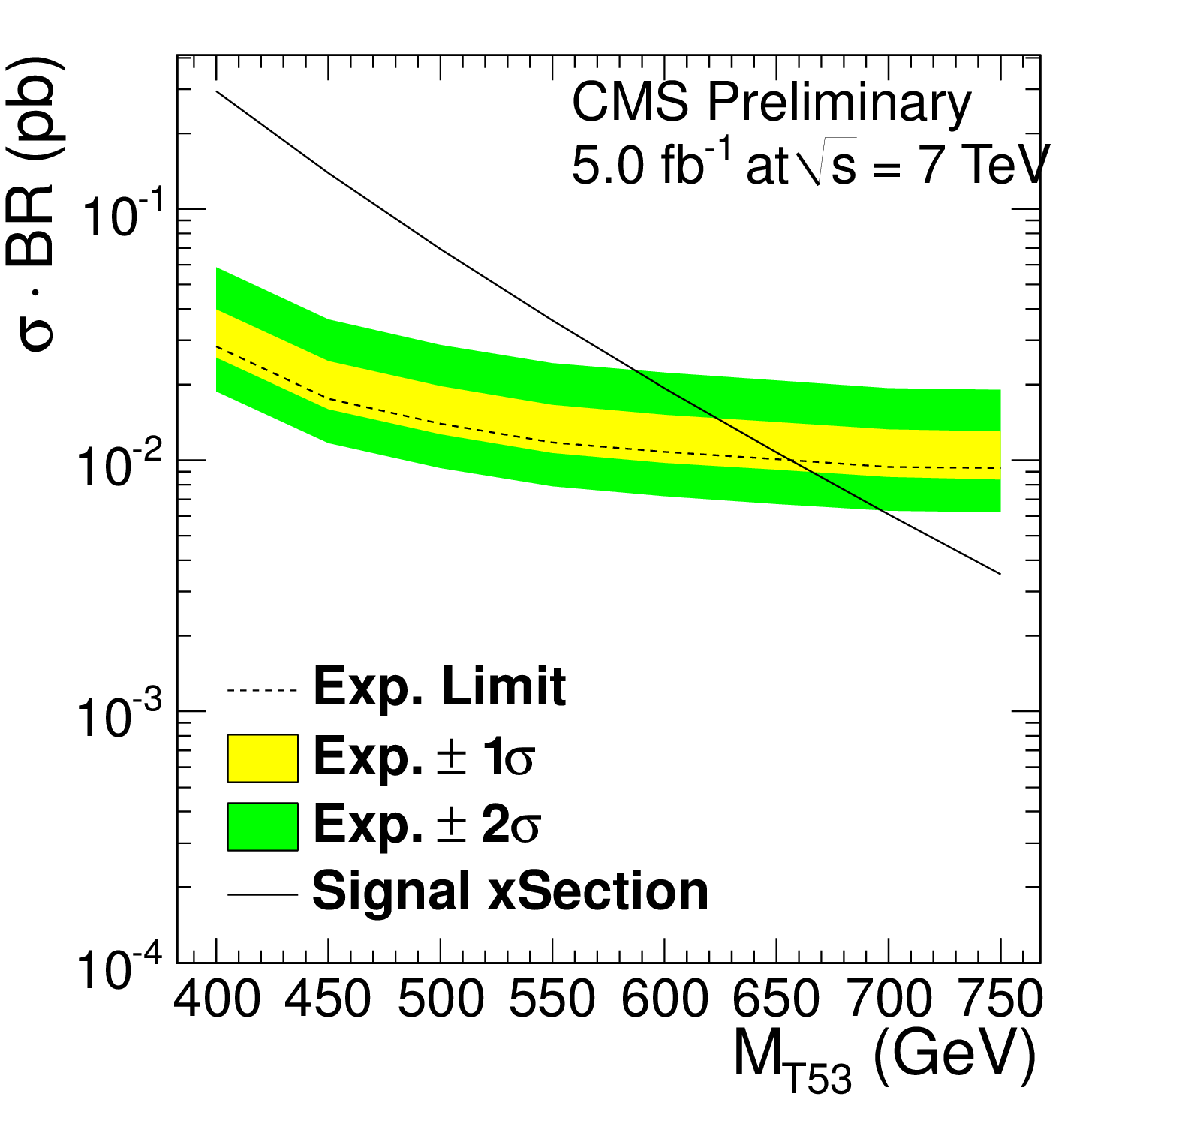
\includegraphics[width=.9\textwidth]{images/pdf/oLimit_limit_macro_4jets_opt_btag_200_350_02}
    \caption{Observed and expected limits for the production cross sections
    of the top partners.}
    \label{fig:limit}
\end{figure}
